\documentclass{beamer}
\usepackage[utf8]{inputenc}

\usetheme{Madrid}
\usecolortheme{default}
\usepackage{amsmath,amssymb,amsfonts,amsthm}
\usepackage{txfonts}
\usepackage{tkz-euclide}
\usepackage{listings}
\usepackage{adjustbox}
\usepackage{array}
\usepackage{tabularx}
\usepackage{gvv}
\usepackage{lmodern}
\usepackage{circuitikz}
\usepackage{tikz}
\usepackage{graphicx}
\usepackage{textcomp}
\usepackage{cancel}
\setbeamertemplate{page number in head/foot}[totalframenumber]

\usepackage{tcolorbox}
\tcbuselibrary{minted,breakable,xparse,skins}



\definecolor{bg}{gray}{0.95}
\DeclareTCBListing{mintedbox}{O{}m!O{}}{%
  breakable=true,
  listing engine=minted,
  listing only,
  minted language=#2,
  minted style=default,
  minted options={%
    linenos,
    gobble=0,
    breaklines=true,
    breakafter=,,
    fontsize=\small,
    numbersep=8pt,
    #1},
  boxsep=0pt,
  left skip=0pt,
  right skip=0pt,
  left=25pt,
  right=0pt,
  top=3pt,
  bottom=3pt,
  arc=5pt,
  leftrule=0pt,
  rightrule=0pt,
  bottomrule=2pt,
  toprule=2pt,
  colback=bg,
  colframe=orange!70,
  enhanced,
  overlay={%
    \begin{tcbclipinterior}
    \fill[orange!20!white] (frame.south west) rectangle ([xshift=20pt]frame.north west);
    \end{tcbclipinterior}},
  #3,
}
\lstset{
    language=C,
    basicstyle=\ttfamily\small,
    keywordstyle=\color{blue},
    stringstyle=\color{orange},
    commentstyle=\color{green!60!black},
    numbers=left,
    numberstyle=\tiny\color{gray},
    breaklines=true,
    showstringspaces=false,
}
%------------------------------------------------------------
%This block of code defines the information to appear in the
%Title page
\title %optional
{4.13.53}
\date{}
%\subtitle{A short story}

\author % (optional)
{Sai Krishna Bakki - EE25BTECH11049}

\begin{document}
\frame{\titlepage}
\begin{frame}{Question}
Lines $L_1 \equiv ax + by + c = 0$ and $L_2 \equiv lx + my + n = 0$ intersect at the point P and make an angle $\theta$ with each other. Find the equation of a line $L$ different from $L_2$ which passes through P and makes the same angle $\theta$ with $L_1$.
\end{frame}

\begin{frame}{Vector Formulation}
    The intersection of lines is given as
\begin{align}
L \equiv L_1 + k L_2 = 0
\end{align}

If $L$ is the reflection of $L_2$ in $L_1$, then for any point \textbf{Q} that lies on $L_2$, its reflection \textbf{R} across the line $L_1$ must lie on $L$.

\begin{align}
 L_1 \equiv ax + by + c = 0 \implies \vec{n}_1^T \vec{x} + c = 0, \vec{n}_1 = \myvec{ a \\ b}.\\
L_2 \equiv lx + my + n = 0 \implies \vec{n}_2^T \vec{x} + n = 0, \vec{n}_2 = \myvec{ l \\ m}. \\
L \equiv (ax+by+c) + k(lx+my+n) = 0 \implies (\vec{n}_1^T \vec{x} + c) + k(\vec{n}_2^T \vec{x} + n) = 0.
\end{align}
\end{frame}
\begin{frame}{Reflection of an Arbitrary Point}
    Let us choose an arbitrary point Q, with position vector $\vec{q}$, that lies on the line $L_2$. The condition that Q is on $L_2$ is:
\begin{align}
\vec{n}_2^T \vec{q} + n = 0
\label{eq:q_on_l2}
\end{align}
Next, we find the position vector $\vec{r}$ for the point R, which is the reflection of Q in the line $L_1$. The standard vector formula for this reflection is:
\begin{align}
\vec{r} = \vec{q} - 2 \brak{ \frac{\vec{n}_1^T \vec{q} + c}{\vec{n}_1^T \vec{n}_1} } \vec{n}_1
\label{eq:reflection_formula}
\end{align}
\end{frame}
\begin{frame}{Applying the Reflection Condition}
    According to our principle, the reflected point R must lie on the line $L$. We substitute the expression for its position vector $\vec{r}$ from \eqref{eq:reflection_formula} directly into the equation for $L$.
\begin{align}
(\vec{n}_1^T \vec{r} + c) + k(\vec{n}_2^T \vec{r} + n) = 0\\
    % Full substitution
     \sbrak{ \vec{n}_1^T \brak{ \vec{q} - 2 \frac{\vec{n}_1^T \vec{q} + c}{\vec{n}_1^T \vec{n}_1} \vec{n}_1 } + c } + k \sbrak{ \vec{n}_2^T \brak{ \vec{q} - 2 \frac{\vec{n}_1^T \vec{q} + c}{\vec{n}_1^T \vec{n}_1} \vec{n}_1 } + n } = 0 
     \end{align}
     \end{frame}
     \begin{frame}{Applying the Reflection Condition}
     \begin{align}
    % Expand terms
    \sbrak{ \vec{n}_1^T\vec{q} - 2 \frac{\vec{n}_1^T \vec{q} + c}{\cancel{\vec{n}_1^T \vec{n}_1}} (\cancel{\vec{n}_1^T\vec{n}_1}) + c } + k \sbrak{ (\vec{n}_2^T \vec{q} + n) - 2 \frac{\vec{n}_1^T \vec{q} + c}{\vec{n}_1^T \vec{n}_1} (\vec{n}_2^T\vec{n}_1) } = 0\\
    % Simplify and use condition
     \sbrak{ \vec{n}_1^T\vec{q} - 2(\vec{n}_1^T \vec{q} + c) + c } + k \sbrak{ 0 - 2 \frac{(\vec{n}_1^T \vec{q} + c)(\vec{n}_1^T\vec{n}_2)}{\vec{n}_1^T \vec{n}_1} } = 0  \\
    % Final simplified form
    -(\vec{n}_1^T \vec{q} + c) - k \sbrak{ 2 \frac{(\vec{n}_1^T \vec{q} + c)(\vec{n}_1^T \vec{n}_2)}{\vec{n}_1^T \vec{n}_1} } = 0
\end{align}
\end{frame}
\begin{frame}{Findng Value Of K}
    Assuming Q is not on $L_1$, the term $(\vec{n}_1^T \vec{q} + c)$ is non-zero, allowing us to divide the entire equation by it:
\begin{align}
-1 - k \sbrak{ \frac{2(\vec{n}_1^T \vec{n}_2)}{\vec{n}_1^T \vec{n}_1} } = 0\\
k = - \frac{\vec{n}_1^T \vec{n}_1}{2(\vec{n}_1^T \vec{n}_2)}
\end{align}
\end{frame}
\begin{frame}{Final Equation}
    Substitute this value of $k$ back into the equation $L_1 + k L_2 = 0$
\begin{align}
L_1 - \frac{\vec{n}_1^T \vec{n}_1}{2(\vec{n}_1^T \vec{n}_2)} L_2 = 0\\
2(\vec{n}_1^T \vec{n}_2) L_1 - (\vec{n}_1^T \vec{n}_1) L_2 = 0
\end{align}
Finally, substituting the algebraic forms for the scalar products:
\begin{itemize}
    \item $\vec{n}_1^T \vec{n}_2 = al + bm$
    \item $\vec{n}_1^T \vec{n}_1 = a^2 + b^2$
\end{itemize}
We arrive at the final equation for the line $L$:
\begin{align}
\boxed{2\myvec{a&b}\myvec{l\\m}\brak{\myvec{a&b}\vec{x}+c} - \myvec{a&b}\myvec{a\\b}\brak{\myvec{l&m}\vec{x}+n} = 0}
\end{align}
\end{frame}
\begin{frame}[fragile]
\frametitle{C Code}
\begin{lstlisting}
#include <stdio.h>

/**
 * @brief Reflects a source line across a mirror line.
 *
 * @param a1, b1, c1 Coefficients of the source line to be reflected.
 * @param a2, b2, c2 Coefficients of the mirror line.
 * @param new_a, new_b, new_c Output pointers for the reflected line's coefficients.
 */
void reflect_line(double a1, double b1, double c1,
                  double a2, double b2, double c2,
                  double* new_a, double* new_b, double* new_c)
{
    // K1 is related to the dot product of the lines' normal vectors.
    double K1 = a1 * a2 + b1 * b2;
\end{lstlisting}
\end{frame}
\begin{frame}[fragile]
\frametitle{C Code}
\begin{lstlisting}
    // K2 is the squared magnitude of the mirror line's normal vector.
    double K2 = a2 * a2 + b2 * b2;

    // Prevent division by zero if the mirror line is invalid (0x + 0y + c = 0).
    if (K2 == 0) {
        *new_a = a1; *new_b = b1; *new_c = c1;
        return;
    }
    
    // Standard formula for line reflection.
    *new_a = 2 * a2 * K1 - a1 * K2;
    *new_b = 2 * b2 * K1 - b1 * K2;
    *new_c = 2 * c2 * K1 - c1 * K2;
}
\end{lstlisting}
\end{frame}
\begin{frame}[fragile]
\frametitle{Python Code Through Shared Output}
\begin{lstlisting}
import ctypes
import os
import matplotlib.pyplot as plt
import numpy as np
from matplotlib.patches import Arc

# --- 1. Compile and Load C Library ---
c_file = "line.c"
so_file = "line.so"
if os.system(f"gcc -shared -o {so_file} -fPIC {c_file}") != 0:
    print(f"Error: C compilation failed. Ensure '{c_file}' exists and is correct.")
    exit()

try:
    line_lib = ctypes.CDLL(f'./{so_file}')
    reflect_line_c = line_lib.reflect_line
    reflect_line_c.argtypes = [
    \end{lstlisting}
\end{frame}
\begin{frame}[fragile]
\frametitle{Python Code Through Shared Output}
\begin{lstlisting}
        ctypes.c_double, ctypes.c_double, ctypes.c_double,
        ctypes.c_double, ctypes.c_double, ctypes.c_double,
        ctypes.POINTER(ctypes.c_double),
        ctypes.POINTER(ctypes.c_double),
        ctypes.POINTER(ctypes.c_double)
    ]
except Exception as e:
    print(f"Error loading shared library: {e}")
    exit()

# --- 2. Define Lines & Find Reflected Line L ---
print("\n--- Problem Setup ---")
a, b, c = 0.0, 1.0, 0.0 # Line L1 (Mirror): y = 0
print(f"Line L1 (Mirror): {a:.1f}x + {b:.1f}y + {c:.1f} = 0")

l, m, n = -0.57, 0.82, 0.0 # Line L2 (Source)
print(f"Line L2 (Source): {l:.2f}x + {m:.2f}y + {n:.1f} = 0")
res_a, res_b, res_c = ctypes.c_double(), ctypes.c_double(), 
\end{lstlisting}
\end{frame}
\begin{frame}[fragile]
\frametitle{Python Code Through Shared Output}
\begin{lstlisting}
ctypes.c_double()
reflect_line_c(l, m, n, a, b, c,
               ctypes.byref(res_a),
               ctypes.byref(res_b),
               ctypes.byref(res_c))
print(f"Found Line L (Reflection): {res_a.value:.2f}x + {res_b.value:.2f}y + {res_c.value:.2f} = 0")

# --- 3. Verify Angles ---
def get_angle(coeffs1, coeffs2):
    a1, b1, _ = coeffs1
    a2, b2, _ = coeffs2
    dot = abs(a1 * a2 + b1 * b2)
    mag1 = np.sqrt(a1**2 + b1**2)
    mag2 = np.sqrt(a2**2 + b2**2)
    
    # SAFETY CHECK: Prevent division by zero if a line is degenerate (0x + 0y + c = 0)
    if mag1 * mag2 == 0:
    \end{lstlisting}
\end{frame}
\begin{frame}[fragile]
\frametitle{Python Code Through Shared Output}
\begin{lstlisting}
        return np.nan # Return "Not a Number" to signify an issue
    
    return np.degrees(np.arccos(dot / (mag1 * mag2)))

angle_L1_L2 = get_angle((a, b, c), (l, m, n))
angle_L1_L = get_angle((a, b, c), (res_a.value, res_b.value, res_c.value))

print("\n--- Angle Verification ---")
print(f"Angle θ between L1 and L2: {angle_L1_L2:.2f}°")

# SAFETY CHECK: Only print and use the angle if it's a valid number
if not np.isnan(angle_L1_L):
    print(f"Angle θ between L1 and L:  {angle_L1_L:.2f}°")
else:
    print("Angle θ between L1 and L: Calculation failed (degenerate line).")
\end{lstlisting}
\end{frame}
\begin{frame}[fragile]
\frametitle{Python Code Through Shared Output}
\begin{lstlisting}
# --- 4. Find Intersection Point P ---
P = (0.0, 0.0)
print(f"\nIntersection Point P is at ({P[0]:.2f}, {P[1]:.2f})")
# --- 5. Generate Plot ---
print("\n--- Generating Plot ---")
plt.style.use('seaborn-v0_8-whitegrid')
fig, ax = plt.subplots(figsize=(8, 8))
x = np.linspace(-3, 3, 400)
def get_y(a_val, b_val, c_val, x_vals):
    if abs(b_val) < 1e-9: return np.full_like(x_vals, np.nan)
    return (-a_val * x_vals - c_val) / b_val
ax.plot(x, get_y(a, b, c, x), 'royalblue', label='Line $L_1$')
ax.plot(x, get_y(l, m, n, x), color='seagreen', label='Line $L_2$')
# Only plot the reflected line if it's valid
if not np.isnan(angle_L1_L):
    ax.plot(x, get_y(res_a.value, res_b.value, res_c.value, x), 'crimson', linestyle='--', label='Reflected Line $L$')
    \end{lstlisting}
\end{frame}
\begin{frame}[fragile]
\frametitle{Python Code Through Shared Output}
\begin{lstlisting}
    # Add angle arcs
    arc1 = Arc(P, 1.5, 1.5, theta1=180-angle_L1_L2, theta2=180, color='gray')
    ax.add_patch(arc1)
    ax.text(0.8, 0.4, r'$\theta$', fontsize=16)
    arc2 = Arc(P, 1.5, 1.5, theta1=0, theta2=angle_L1_L, color='gray')
    ax.add_patch(arc2)
    ax.text(-0.9, 0.4, r'$\theta$', fontsize=16)

ax.plot(P[0], P[1], 'ko', markersize=10, label='Intersection Point P')

ax.set_title('Line Reflection', fontsize=16)
ax.set_xlabel('x-axis'), ax.set_ylabel('y-axis')
ax.legend(), ax.axis('equal'), ax.set_xlim(-3, 3), ax.set_ylim(-3, 3)
plt.show()
\end{lstlisting}
\end{frame}
\begin{frame}[fragile]
\frametitle{Python Code}
\begin{lstlisting}
import numpy as np
import matplotlib.pyplot as plt
import matplotlib.patches as patches
from libs.funcs import * 

P = np.array([[0], [0]])
theta_deg = 35
theta_rad = np.deg2rad(theta_deg)

# --- 2. Construct the Lines Geometrically ---
n1 = np.array([[0], [1]])
n2 = rotmat(theta_rad) @ n1
n_L = rotmat(-theta_rad) @ n1

# --- 3. Generate Points for Plotting ---
m1 = omat @ n1
m2 = omat @ n2
m_L = omat @ n_L
line_length = 5
\end{lstlisting}
\end{frame}
\begin{frame}[fragile]
\frametitle{Python Code}
\begin{lstlisting}
x_L1 = line_dir_pt(m1, P, -line_length, line_length)
x_L2 = line_dir_pt(m2, P, -line_length, line_length)
x_L = line_dir_pt(m_L, P, -line_length, line_length)

# --- 4. Create a Clean and Clear Plot ---
plt.style.use('seaborn-v0_8-whitegrid')
fig, ax = plt.subplots(figsize=(10, 10))

ax.plot(x_L1[0, :], x_L1[1, :], color='royalblue', linewidth=2.5, label='Line $L_1$')
ax.plot(x_L2[0, :], x_L2[1, :], color='seagreen', linewidth=2.5, label='Line $L_2$')
ax.plot(x_L[0, :], x_L[1, :], color='crimson', linestyle='--', linewidth=2.5, label='Reflected Line $L$')
ax.plot(P[0], P[1], 'o', color='black', markersize=9, label='Intersection Point P')

# --- 5. Add Line Equation Labels ---
eq1 = "$y = 0$"
\end{lstlisting}
\end{frame}
\begin{frame}[fragile]
\frametitle{Python Code}
\begin{lstlisting}
eq2 = f"${n2[0,0]:.2f}x + {n2[1,0]:.2f}y = 0$"
eqL = f"${n_L[0,0]:.2f}x + {n_L[1,0]:.2f}y = 0$"

ax.text(1.5, 0.15, eq1, color='royalblue', fontsize=12, va='bottom', backgroundcolor='white')
ax.text(-2.4, 1.7, eq2, color='seagreen', fontsize=12, rotation=-theta_deg, va='bottom', backgroundcolor='white')
ax.text(-2.4, -2.0, eqL, color='crimson', fontsize=12, rotation=theta_deg, va='bottom', backgroundcolor='white')

# --- 6. Add Angle Annotations ---
arc_radius = 1.5
arc1 = patches.Arc(P.flatten(), arc_radius, arc_radius, angle=90, 
                   theta1=0, theta2=theta_deg, color='gray', linewidth=2)
arc2 = patches.Arc(P.flatten(), arc_radius, arc_radius, angle=90, 
                   theta1=-theta_deg, theta2=0, color='gray', linewidth=2)
ax.add_patch(arc1)
\end{lstlisting}
\end{frame}
\begin{frame}[fragile]
\frametitle{Python Code}
\begin{lstlisting}
ax.add_patch(arc2)
ax.text(0.8 * np.cos(np.deg2rad(18)), 0.8 * np.sin(np.deg2rad(18)), r'$\theta$', fontsize=18)
ax.text(0.8 * np.cos(np.deg2rad(-18)), 0.8 * np.sin(np.deg2rad(-18)), r'$\theta$', fontsize=18)

# --- 7. Finalize and Show the Plot ---
ax.set_title(f'Line Reflection with Angle $\\theta = {theta_deg}^\\circ$', fontsize=16)
ax.set_xlabel('x-axis', fontsize=12)
ax.set_ylabel('y-axis', fontsize=12)
ax.set_aspect('equal', adjustable='box')
lim = 2.8
ax.set_xlim(-lim, lim)
ax.set_ylim(-lim, lim)
ax.legend(fontsize=11)

plt.show()
\end{lstlisting}
\end{frame}
\begin{frame}{Plot By C code and Python Code}
    \begin{figure}
    \centering
    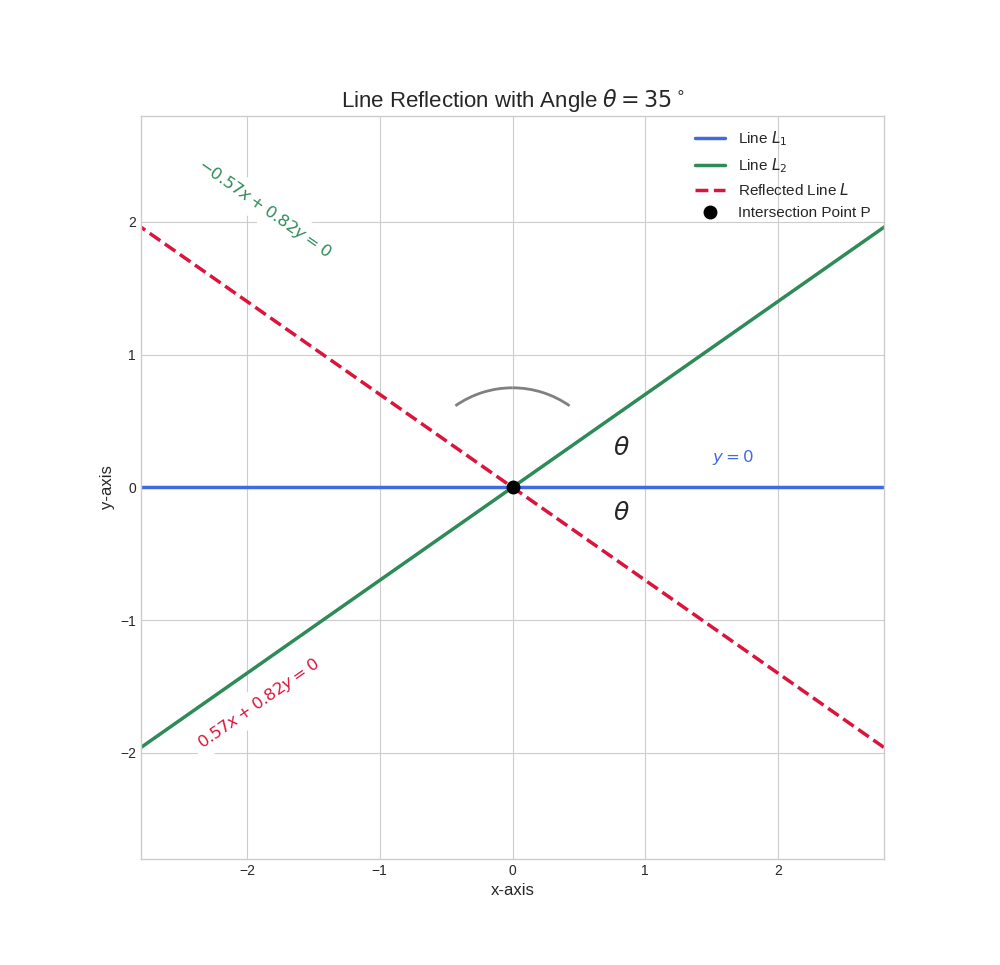
\includegraphics[width=0.7\columnwidth]{figs/Figure_1.png}
    \label{fig:placeholder}
    \caption{1}
\end{figure}
\end{frame}
\end{document}